\documentclass[a4paper,12pt,titlepage=true, ngerman]{scrartcl}
%\usepackage{ngerman}, 
%\usepackage[ngerman]{babel}


\usepackage[utf8]{inputenc}
\usepackage[ngerman]{babel}
\usepackage[babel, german=quotes]{csquotes}
\usepackage{hyperref}
\usepackage{graphicx}

\usepackage{scrhack}
\KOMAoptions{BCOR=8mm}
%\KOMAoptions{toc=flat}
% \KOMAoptions{toc=graduated, toc=bibliography}

% \renewcommand*\sectfont{\rmfamily\mdseries\scshape}
\setkomafont{section}{\rmfamily\bfseries\LARGE}
% \setkomafont{sectionentry}{\rmfamily\bfseries\scshape\Large}
\setkomafont{subsection}{\rmfamily\bfseries\Large}
\setkomafont{subsubsection}{\rmfamily\bfseries\large}
%\setkomafont{chapter}{\rmfamily\bfseries\scshape\huge}
%  \setkomafont{partentry}{\rmfamily\bfseries\scshape}
% \setkomafont{chapterentry}{\rmfamily\bfseries\scshape}
\setkomafont{partentry}{\rmfamily\bfseries\scshape}
\setkomafont{part}{\rmfamily\bfseries\scshape\huge}
\setkomafont{partnumber}{\rmfamily\bfseries\scshape\huge}
\setkomafont{partentrypagenumber}{\rmfamily\bfseries\scshape}

\setkomafont{descriptionlabel}{\bfseries}

%  scrhack to fuck float error message

%%%%  for page head and foot %%%%%%%
\usepackage[automark]{scrpage2}
\pagestyle{scrheadings}
\KOMAoptions{headsepline=true}
\setheadsepline{.4pt}
\setkomafont{pageheadfoot}{\normalfont\normalcolor\upshape} 

\setcounter{tocdepth}{3}
\setcounter{secnumdepth}{4}

\usepackage[T1]{fontenc} % to make Sa\"ibi searchable
\usepackage[protrusion=true,expansion=true]{microtype}
% \usepackage{microtype}
% \usepackage{setspace}\setstretch{1.2}



% \usepackage{lmodern} 


%  \usepackage{palatino}\linespread{1.05}
 \usepackage{mathpazo}\linespread{1.05}  
\usepackage[scaled=.95]{helvet}
   \usepackage{courier}
   \usepackage[scaled]{berasans}
 
% \usepackage[bitstream-charter]{mathdesign}  %%%%%%%%%%%%%%%%%%%%%  FINAL VERSION %%%%%%%%%%%%%%%%%%%%%%%%%%%%%%%


\usepackage[style=authoryear,
 maxnames=1,
  maxbibnames=99,                  %%%%%%%%     TODO  activate
 uniquename=init
]{biblatex}
\bibliography{literature.bib}





\usepackage{calc}
\usepackage{ifthen}

\usepackage{tikz}
\usetikzlibrary{shapes,arrows}

\tikzstyle{task} = [diamond, draw, fill=green!20, 
    text width=4.5em, text badly centered, node distance=2cm, inner sep=0pt]
\tikzstyle{comp} = [rectangle, draw, fill=blue!20, 
    text width=5em, text centered, rounded corners, minimum height=4em, node distance=2cm]
\tikzstyle{line} = [draw, -latex']
\tikzstyle{line2} = [draw, double, -latex']
\tikzstyle{human} = [draw, ellipse,fill=red!20, text width=5em, text centered, node distance=2cm,
    minimum height=3em]
\tikzstyle{decision} = [diamond, draw, fill=green!20, 
    text width=4.5em, text badly centered, node distance=3cm, inner sep=0pt]
\tikzstyle{block} = [rectangle, draw, fill=blue!20, 
    text width=5em, text centered, rounded corners, minimum height=4em]
\tikzstyle{cloud} = [draw, ellipse,fill=red!20, text width=5em, text centered, node distance=3cm,
    minimum height=2em]

% % Pie chart
\newcommand{\slice}[4]{
  \pgfmathparse{0.5*#1+0.5*#2}
  \let\midangle\pgfmathresult

  % slice
  \draw[thick,fill=black!10] (0,0) -- (#1:1) arc (#1:#2:1) -- cycle;

  % outer label
  \node[label=\midangle:#4] at (\midangle:1) {};

  % inner label
  \pgfmathparse{min((#2-#1-10)/110*(-0.3),0)}
  \let\temp\pgfmathresult
  \pgfmathparse{max(\temp,-0.5) + 0.8}
  \let\innerpos\pgfmathresult
  \node at (\midangle:\innerpos) {#3};
}

\usepackage{bchart}


\usepackage{setspace}
\onehalfspacing

% \usepackage{framed}

\usepackage{graphicx}

\usepackage{ownstyle}

\usepackage{cleveref}

\title{Dokumentation zur Arbeit von Gruppe 2 im Projekt ''Praxis der Digital Humanities''} % title
\author{Clemens Ahrens}

\begin{document}
\begin{titlepage}

\begin{center}

\vspace*{100pt}

\large\textbf{Dokumentation zur Arbeit von Gruppe 2 im Projekt ''Praxis der Digital Humanities''}% title

\vfill

Schriftliche Dokumentation

im Seminar

\emph{Praxis der Digital Humanities}


Leitung:

\textbf{Prof.\ Dr.\ Caroline Sporleder}% leitung

WiSe 2014/2015% semester

\bigskip

an der Universität Trier

Fachbereich II

\bigskip

\bigskip

Verfasser:

\textbf{Chris} %TODO

Matrikelnummer:

xxxxxx

\textbf{Andre} %TODO

Matrikelnummer:

xxxxxx

\textbf{Clemens Ahrens}

Matrikelnummer:

1116125

% \bigskip

% \vfill

\end{center}

\end{titlepage}

\microtypesetup{protrusion=false}
 \tableofcontents%[liststotoc]
\microtypesetup{protrusion=true}

% \newpage
% \listoffigures
% \listoftables

\newpage

% !TEX encoding = UTF-8
\subsubsection{Steckbrief}
Analysiert wurde \href{http://www.bart-anaphora.org/}{BART} in der Version 2.0, 
wie sie \href{http://www.bart-anaphora.org/release/bart-2.0.tar.gz}{hier} zu finden 
ist.
Es stehen dem Nutzer zwei Modi zur Nutzung zur Verfügung.
\begin{itemize}
\item BART-WebServer als end-to-end Blackbox Lösung
\item BART-full zum Trainieren eines neuen Modells
\end{itemize}
Erstere erzeugt aus einem Rohtext-Input einen Output, 
wie er in Abb.\ref{bart_webUI_output} zu sehen ist.
Hierfür werden verschiedene Verarbeitungsschritte durchgeführt. 
Diese analysieren jeweils unterschiedliche Ebenen in Syntax und Semantik. 
Beispielhaft hierfür soll der Output der WebServer-Anwendung für die Wortebene in 
Listing\ref{output:bart_word} stehen.

\begin{lstlisting}[label=output:bart_word, name=words.xml, language=xml, caption=BART-Output der Wortebene]
?xml version="1.0" encoding="UTF-8"?>
<!DOCTYPE words SYSTEM "words.dtd">
<words>
  <word id="word_1">Late</word>
  <word id="word_2">in</word>
  <word id="word_3">the</word>
  <word id="word_4">afternoon</word>
  ...
</words>
\end{lstlisting}
Der Output auf Koreferenzebene im XML-Format ist exemplarisch in 
Listing\ref{output:bart_response} dargestellt.
Hierbei ist die Koreferenzkette ,,a low man'' aus Abb.\ref{bart_webUI_output} in dem 
Attribut \lstinline[language=XML]{coref_set="set_4"} kodiert.

\begin{lstlisting}[label=output:bart_response, name=XXX_response_level.xml, language=xml, caption=BART-Output der Koreferenzebene]
<markables>
  ...
  <markable id="markable_51" span="word_120..word_122" coref_set="set_4" min_ids="word_120..word_122" mmax_level="response"/>
  <markable id="markable_13" span="word_128" coref_set="set_4" dir_antecedent="markable_51" mmax_level="response"/>
  <markable id="markable_0" span="word_128..word_129" coref_set="set_0" min_ids="word_128..word_129" mmax_level="response"/>
  ...
</markables>
\end{lstlisting}

\begin{figure}[ht]
\begin{center}
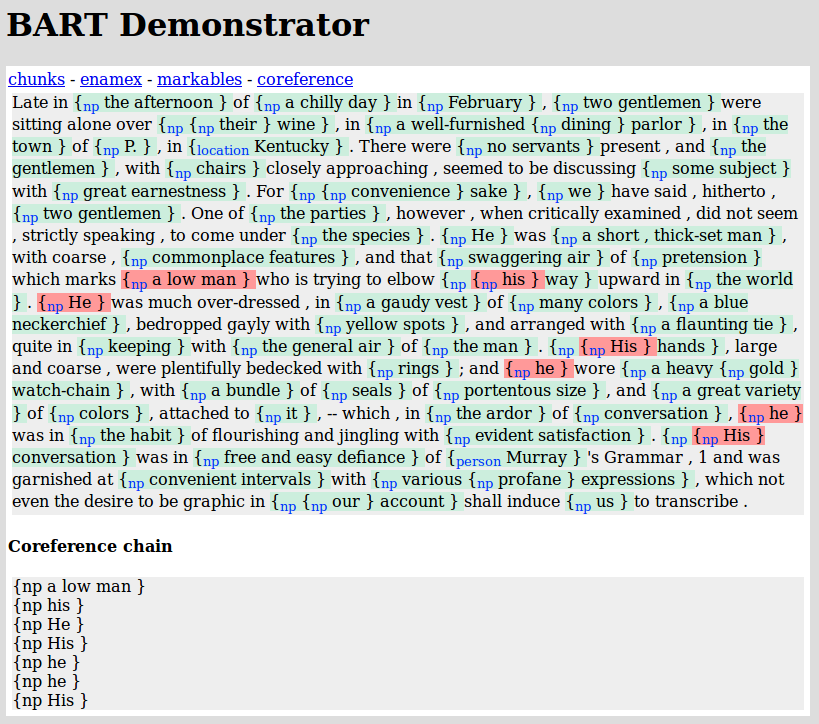
\includegraphics[width=12cm]{./img/cle/bart_webUI_output.png}
 % bart_webUI_output.png: 819x724 pixel, 72dpi, 28.89x25.54 cm, bb=0 0 819 724
\caption{BART 2.0: Output für WebInterface der Blackbox Version}
\label{bart_webUI_output}
\end{center}
\end{figure}

\subsubsection{Probleme}

\noindent
Neben der Blackbox-Version bietet BART noch eine Terminalapplikation, 
die zum Trainieren neuer Modelle genutzt werden kann.
Hierfür stehen verschiedene interne Konfigurationsdateien zur Verfügung,
die sich jedoch auf die Weiterverarbeitung beziehen und nicht den erwarteten
Input modifizieren.

Da im Projekt die Verarbeitung von Output des Stanford Parsers gewünscht war,
und wir daher auch innerhalb unserer Gruppe von der Verwendung des MMAX-Formats 
Abstand genommen haben, wurde von der Konvertierung in dieses Format abgesehen.
Eine erste Analyse der Koreferenzketten, die die WebServer-Version von BART ausgab,
unterstützte diese Entscheidung ebenfalls.



% !TEX encoding = UTF-8
\section{clemens\_code}\label{clemens_code}
%TODO headings for lstlistings
\lstset{language=Java} 
\begin{lstlisting}[caption=Main-Klasse der BuildIndex,label=code:Coref, name=Coref.java] 
import java.util.ArrayList;
import java.util.Map;

public class Coref {
	ArrayList<String> inFiles;
	String outFile;

	// parser for inputs
	void parseArgs(String[] args) {
		Integer iIdx = null;
		Integer oIdx = null;
		inFiles = new ArrayList<String>();

		// input must come before output ---
		for (int i = 0; i < args.length; i++) {
			if (args[i].equals("-i")) {
				iIdx = new Integer(i);
			} else if (args[i].equals("-o")) {
				oIdx = new Integer(i);
			}
		}
		if (iIdx != null & oIdx != null) {
			outFile = args[oIdx + 1];
			for (int i = iIdx + 1; i < oIdx; i++) {
				inFiles.add(args[i]);
			}
		} else {
			System.out.println("Usage: " + "\n"
					+ "java Coref -i <XmlFile> -o <NewFile>" + "\n"
					+ "Example (Linux): " + "\n"
					+ "java Coref -i ../Input/*.xml -o ../output.xml");
			System.exit(-1);
		}
	}

	public static void main(String[] args) {
		Coref coref = new Coref();
		coref.parseArgs(args);

		OutputWriter outputWriter = new OutputWriter(coref.getOutFile());

		// for each input XML: Analyze, build Maps of coreferences, pass to output XML
		try {
			for (String inFile : coref.getInFiles()) {
				InputAnalyzer inputAnalyzer = new InputAnalyzer(inFile);

				Map<String, Coreference> coreferences = inputAnalyzer
						.extractCoreferences();

				outputWriter.addCoreferences(coreferences);
			}
		} catch (Exception e) {

			e.printStackTrace();
		}

		// create output XML
		outputWriter.writeToFile();

	}

	public ArrayList<String> getInFiles() {
		return inFiles;
	}

	public String getOutFile() {
		return outFile;
	}
}
\end{lstlisting} 

\begin{lstlisting}[caption=Coreference-Klasse,label=code:Coreference, name=Coreference.java]
public class Coreference {
	String text;
	String chapId;
	Integer corefId;

	public Coreference(String text, String chapId, Integer corefId) {
		this.text = text;
		this.chapId = chapId;
		this.corefId = corefId;
	}

	public String getText() {
		return text;
	}

	public void setText(String text) {
		this.text = text;
	}

	public String getChapId() {
		return chapId;
	}

	public void setChapId(String chapId) {
		this.chapId = chapId;
	}

	public Integer getCorefId() {
		return corefId;
	}

	public void setCorefId(Integer corefId) {
		this.corefId = corefId;
	}

}
\end{lstlisting}

\begin{lstlisting}[caption=InputAnalyzer-Klasse,label=code:InputAnalyzer, name=InputAnalyzer.java]
import java.io.File;
import java.io.IOException;
import java.util.ArrayList;
import java.util.HashMap;
import java.util.List;
import java.util.Map;

import org.jdom.Document;
import org.jdom.Element;
import org.jdom.JDOMException;
import org.jdom.input.SAXBuilder;

public class InputAnalyzer {

	File infile;
	
	public InputAnalyzer(String filename) throws Exception {
		infile = new File(filename);
		if (!infile.exists()) {
			throw new Exception("File " + filename + " not found");
		}
	}

	public Map<String, Coreference> extractCoreferences() {
		Map<String, Coreference> map = new HashMap<String, Coreference>();

		// aufrufen des builders pro input
		SAXBuilder builder = new SAXBuilder();
		try {
			Document doc = builder.build(infile);

			// ---- Create list of <coreferences> & extract chapID
			Element root = doc.getRootElement();

			// extract argument chapter ID for output document
			String chapID = root.getAttribute("id").getValue();

			// jump to necessary level of sub elements
			Element corefs = root.getChild("coreferences");

			@SuppressWarnings("unchecked")
			List<Element> listcoref = corefs.getChildren("coreference");
			for (Element coref : listcoref) {
				String corefID = coref.getAttribute("id").getValue();

				// create list of mentions for each coreference chain
				@SuppressWarnings("unchecked")
				List<Element> listmention = coref.getChildren("mention");
				for (Element mention : listmention) {
					if (null == mention)
						continue;
					
					// search for "representative" mention
					String s = mention.getAttributeValue("representative");
					if (null == s || !s.equals("true"))
						continue;

					// extract XML element <text> for output document
					String text = mention.getChildText("text");

					// build new Coreference element with needed attributes &
					// turn corefID to Integer
					Coreference coreference = new Coreference(text, chapID,
							Integer.parseInt(corefID));
					map.put(text, coreference);

				}
			}
		} catch (JDOMException | IOException e) {
			// TODO Auto-generated catch block
			e.printStackTrace();
		} catch (NumberFormatException e) {
			System.err.println("Error while parsing corefID: \n"
					+ e.getMessage());
		}

		return map;

	}

}
\end{lstlisting}
\begin{lstlisting}[caption=OutputWriter-Klasse der BuildIndex,label=code:OutputWriter, name=OutputWriter.java]
import java.io.File;
import java.io.FileOutputStream;
import java.io.IOException;
import java.util.ArrayList;
import java.util.HashMap;
import java.util.Map;
import java.util.Set;

import org.jdom.Document;
import org.jdom.Element;
import org.jdom.output.Format;
import org.jdom.output.XMLOutputter;

public class OutputWriter {

	File outFile;
	Map<String, ArrayList<Coreference>> multiMap;

	public OutputWriter(String filename) {
		outFile = new File(filename);
		multiMap = new HashMap<String, ArrayList<Coreference>>();
	}

	public void addCoreferences(Map<String, Coreference> coreferences) {
		Set<String> keySet = coreferences.keySet();
		for (String key : keySet) {
			// create ArrayList if key not already existent
			if (!multiMap.containsKey(key)) {
				multiMap.put(key, new ArrayList<Coreference>());
			}
			// add coreference for key to ArrayList in multiMap for key
			multiMap.get(key).add(coreferences.get(key));
		}
	}

	public void writeToFile() {
		// create output element, which will be turned to output XML later
		Document outputdoc = new Document(new Element("root"));

		// write basic elements
		Element chains = new Element("chains");
		Element outroot = outputdoc.getRootElement();
		outroot.addContent(chains);
		// ---- create sub elements for each coref in outputdoc
		for (String key : multiMap.keySet()) {
			Element chain = new Element("chain");
			chains.addContent(chain);
			chain.setAttribute("text", key);

			for (Coreference coreference : multiMap.get(key)) {
				Element coref = new Element("coreference");
				Element chapter = new Element("chapter");
				Element id = new Element("id");

				chain.addContent(coref);
				coref.addContent(id);
				id.addContent(coreference.getCorefId().toString());
				coref.addContent(chapter);
				chapter.addContent(coreference.getChapId());

			}
		}

		// format output XML file
		XMLOutputter outp = new XMLOutputter();
		outp.setFormat(Format.getPrettyFormat());

		// ---- Write the complete result document to output XML file ----
		try {
			outp.output(outputdoc, new FileOutputStream(outFile));
		} catch (IOException e) {
			System.err.println("Error writing output file.");
			e.printStackTrace();
		}
	}
}
\end{lstlisting}
 

% \input{generierung}

% \input{normalisierung}

% \input{evaluierung}

% \input{ausblick}

% \printshorthands[title=Abkürzungsverzeichnis]
\printbibliography[title=Literaturverzeichnis, heading=bibintoc]
\newpage
\listoffigures
\listoftables
\newpage

\thispagestyle{empty}
\subsection*{Erklärung}
Hiermit erkläre ich, dass ich die Hausarbeit selbstständig
verfasst und keine anderen als die angegebenen Quellen und Hilfsmittel benutzt
und die aus fremden Quellen direkt oder indirekt übernommenen Gedanken als
solche kenntlich gemacht habe.

Die Arbeit habe ich bisher keinem anderen Prüfungsamt in gleicher oder
vergleichbarer Form vorgelegt. Sie wurde bisher nicht veröffentlicht.


\vspace{3cm}
\begin{center}
(Datum) \hspace{8cm} (Unterschrift)
\end{center}
% \left Datum
% \right Unterschrift

\end{document}